\section{空间解析几何}

思考一下, 在高中的时候, 对于直线与平面的关系, 大致可以分为如下的几个阶段: 
\begin{itemize}
	\item 初中的时候, 我们学习了$y=kx+b$来表示直线;
	\item 高中的时候, 我们拓展了视野, 注意到了$Ax+By+C=0$也可以表示一个直线. 
	\item 再后来, 参数方程的知识告诉我们可以用$\begin{cases}
		x=\varphi(t)\\
		y=\psi(t)
	\end{cases}$表示. 
	\item 在圆锥曲线的一节中, 根据方程与曲线, 我们知道了平面曲线上的点可以与方程一一对应. 
\end{itemize}

现在, 我们试图对于上述探索历程进行拓展: 是不是可以把空间中的图形与方程或不等式联系起来? 

\begin{tool}
	像在高中数学的教科书中演示的那样, 我们可以用辅助工具Geogebra 3D或者Mathematica来辅助观察. 
	
	Geogebra是互联网上的一个小程序, 可以在\url{https://www.geogebra.org/3d}自己玩一玩. 
	
	Wolfram Alpha 是一个智能的计算机求解程序的工具. 如果你们的学校有幸购买了这个软件的话, 可以下载下来使用\texttt{plot3d}指令绘制三维图像. 
\end{tool}

\subsection{平面与空间的相似与不同}

在学习《数学必修二》中的立体几何的时候, 我们会发现, 两个直线之间的关系不只有平行和垂直了. 多出来了一个``异面''的情形. 然而, 当我们探讨平面与平面之间的关系的时候, 就只有``平行'' 与``垂直''两种情形. 这就暗示了直线与直线的情形在空间中和平面与平面的行为很像. 

同样, 我们发现在处理直线与平面的问题的时候, 很多时候有``自由度''. 毕竟空间的维数多出来了一维. 这些内容我们可以如何刻画? 

\subsection{从直线与平面开始}

我们发现, 在平面里面的直线可以由一个方程$Ax+By+C=0$唯一决定. 所有的解$(x,y)$这样一系列的点构成了整条直线. 

\begin{bonus}
	我们应该如何刻画直线是``直的''这一属性? 刻画的方法可否较为容易地推广到三维(甚至更高维度)的情形? 
\end{bonus}

我们发现, 用坐标和向量的观念是具有泛化(generlization)能力的. 于是我们可以借助上面的一些内容来表示平面. 

我们先猜测既然是三维空间, 那么自然多引入一个$Cz$, 让作图机画一下看一看是不是这样的: 在这里, 我选用gnuplot这一个命令行工具为我画图. 请参看图\ref{fig:plane-in-space}. 我的命令是绘制$2x+3y-z=0$. 其果然是一个平面! 

\begin{figure*}
	\begin{center}
		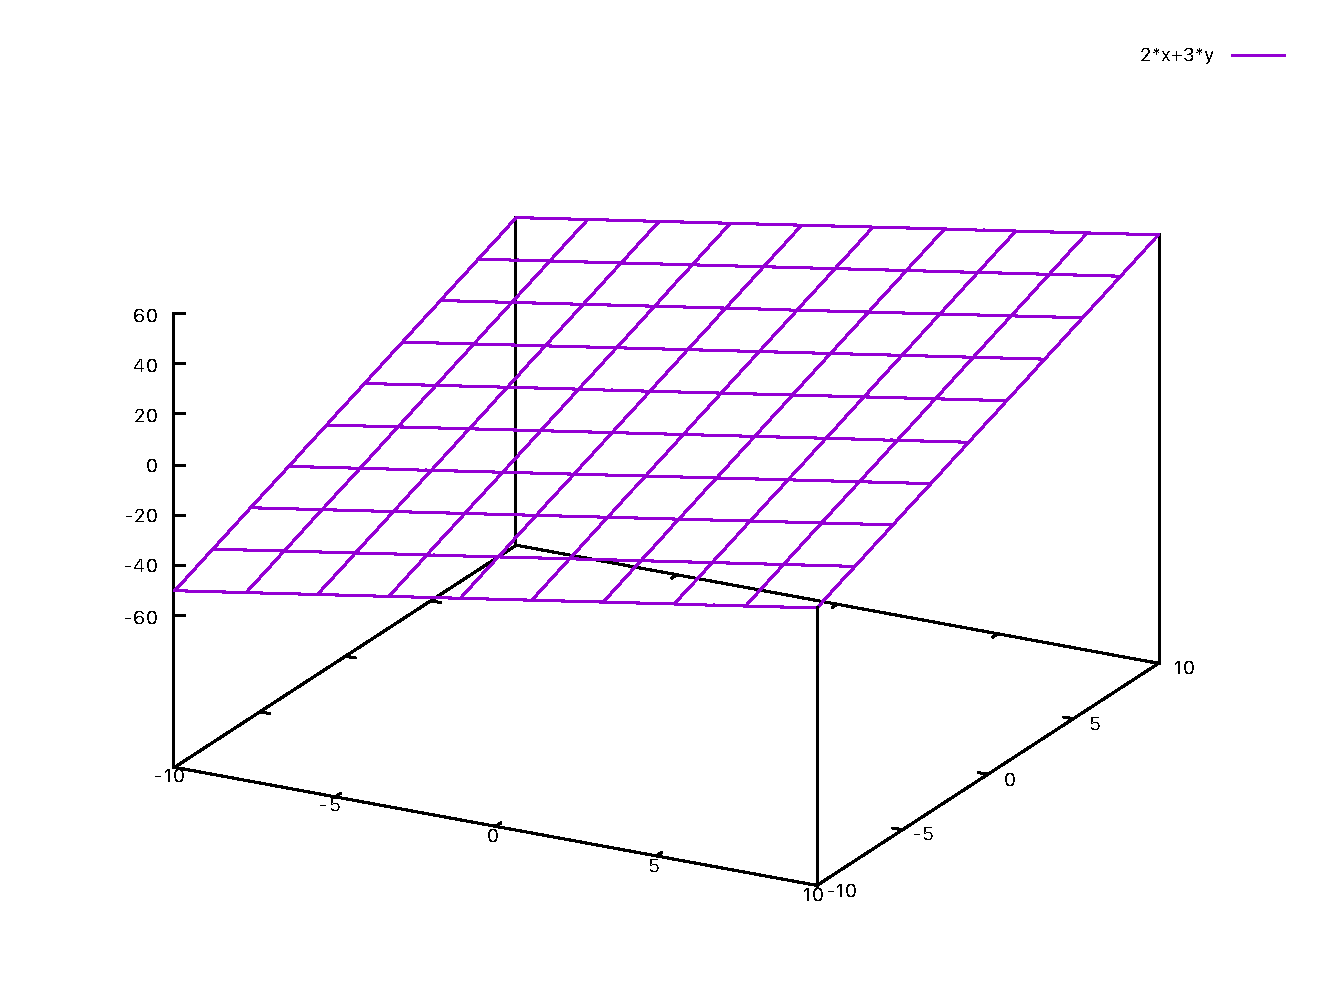
\includegraphics[scale=0.5]{space-ana-geo/line-look.pdf}
	\end{center}
	\label{fig:plane-in-space}
	\caption{坐标系中平面的内容}
\end{figure*}

